\documentclass[10pt,xcolor=dvipsnames,serif,professionalfont]{beamer} % " professionalfont " option
\usepackage{pifont,manfnt}
\usepackage{booktabs}
\usepackage[T1]{fontenc}
\usepackage{mathpazo}
\usepackage{eulervm}
\usepackage{tikz}
\linespread{1.05}
\usepackage{xspace}
\usepackage{apacite}
\usepackage{rotating}
\usepackage{multirow}
\input{andrews_commands}
\setbeamerfont{title}{family=\it}
\setbeamerfont{frametitle}{family=\it}

\usepackage{tikz}
\usetikzlibrary{trees}

\usepackage{amssymb,latexsym,amsmath,amsfonts,amscd}

\usecolortheme[named=Gray]{structure} 
\setbeamercolor{titlelike}{fg=black!60!red}
\definecolor{Mygrey}{gray}{0.75}


\graphicspath{{../images/}}

\title{Introducing Generalized Linear Models}
\author[Andrews]{Mark Andrews}
\date{}


\DeclareSymbolFont{legacymaths}{OT1}{cmr}{m}{n}
\DeclareMathAccent{\dot}     {\mathalpha}{legacymaths}{95}
\DeclareMathAccent{\bar}     {\mathalpha}{legacymaths}{22}
\DeclareMathAccent{\tilde}     {\mathalpha}{legacymaths}{126}


\begin{document}
{
\begin{frame}
   \titlepage
\end{frame}
}

\begin{frame}%[<+->]
\frametitle{Logistic regression as a generalization of linear regression}
\begin{itemize}
\item If $y$ is continuous, it may be appropriate to model $y$ as a noisy linear function of $x$, i.e. 
\[ y = \alpha + \beta x + \epsilon.\]
\item If $y \in \{0,1\}$, then we can model the \emph{probability} that $y$ takes the value 1 as an \emph{inverse logit} function of $x$
\[ \Prob{y=1} = \phi(\alpha + \beta x) = \frac{1}{1+e^{-\alpha - \beta x}}.\]
\end{itemize}
\end{frame}

\begin{frame}%[<+->]
\frametitle{Logistic regression as generalized linear regression}
\begin{itemize}
\item In linear-Gaussian regression, we assume the following:
\[
y_i \sim N(\mu_i,\sigma^2),\quad\text{where}\ \mu_i = \alpha+ \beta x_{i} .
\]
\item By contrast, in binary logistic regression we assume the following:
\[
	y_i \sim \textrm{Bernoulli}(p_i),\quad\text{where}\ p_i = \phi(\alpha + \beta x) = \frac{1}{1 + e^{-\alpha- \beta x_{i}}}.
\]
\end{itemize}
\end{frame}

\begin{frame}
\frametitle{Alternative description of logistic regression}
\begin{itemize}
\item Rather than viewing $\Prob{y=1}$ as a transformed linear function of $x$, we can view
\[\log \left( \frac{\Prob{y=1}}{1-\Prob{y=1}}\right),\]
as a linear function of $x$. 
\item In other words,
\begin{align*}
y_i &\sim \textrm{Bernoulli}(p_i),\quad\text{where}\ \log\left(\frac{p_i}{1-p_i}\right) = \alpha + \beta x_i .
\end{align*}
\end{itemize}
\end{frame}

\begin{frame}
\frametitle{Logit and inverse-logit function}
\begin{itemize}
\item The two regression models, i.e. 
\begin{align*}
y_i &\sim \textrm{Bernoulli}(p_i),\quad\text{where}\ p_i = \frac{1}{1 + e^{-\alpha- \beta x_{i}}},
\intertext{and}
y_i &\sim \textrm{Bernoulli}(p_i),\quad\text{where}\ \log\left(\frac{p_i}{1-p_i}\right) = \alpha + \beta x_i .
\end{align*}
are identical.
\end{itemize}
\end{frame}



\begin{frame}
\frametitle{The Poisson Distribution}
\begin{itemize}
\item The Poisson distribution is a discrete probability distribution over the non-negative integers $0,1,2 \ldots$.
\begin{center}
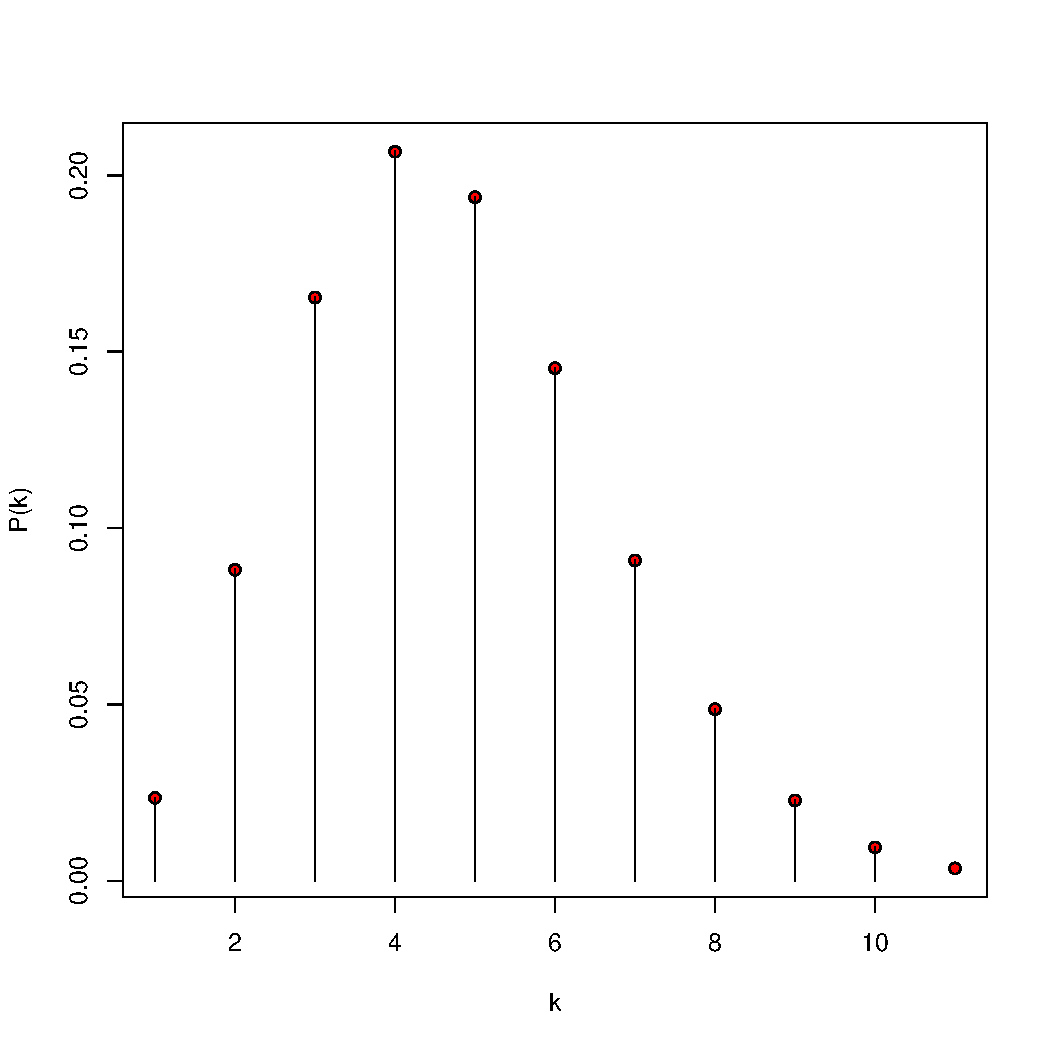
\includegraphics[width=.55\textwidth]{figs/poisson_375.pdf}
\end{center}
%\begin{center}
%\input{poissonplot}
%\end{center}

%\item It is used to model the probability of a given number of events occurring in a fixed interval of time, e.g. the number of trams that pass Chaucer during this class.
\end{itemize}
\end{frame}


\begin{frame}
\frametitle{The Poisson Distribution}
\begin{itemize}
\item The Poisson distribution is used to model the probability of a given number of events occurring in a fixed interval of time, e.g. the number of trams that pass Chaucer during this class.
\item It has a single parameter $\lambda$, known as the \emph{rate}.
\item If $x$ is a Poisson random variable whose, its probability mass function is 
\[\Prob{x=k\given \lambda} = \frac{e^{-\lambda}\lambda^k}{k!}.\]
\end{itemize}
\end{frame}
\begin{frame}
\frametitle{Poisson Regression}
\begin{itemize}
\item In any regression problem, our data are $(y_1,x_1), (y_2,x_2) \ldots (y_n,x_n)$, where each $y_i$ is modelled as a stochastic function of $x_i$.
\item In Poisson regression, we assume that each $y_i$ is a Poisson random variable rate $\lambda_i$ and 
\[\log(\lambda_i) = \beta_0 + \sum_{k=1}^K \beta_k x_{ki},\]
or equivalently 
\[\lambda_i = e^{\beta_0 + \sum_{k=1}^K \beta_k x_{ki}}.\]
\end{itemize}
\end{frame}


\begin{frame}
\frametitle{Poisson Regression}
\begin{itemize}
\item As an example of Poisson regression, we can look at the number visits to a doctor in a fixed period as a function of predictors such as gender.
\item Using a data-set of over 5000 people, we estimate (using mle) that 
\[\log(\lambda_i) = 1.65 + 0.43\times x_i \]
where $x_i=1$ for a female, and $x_i=0$ for a male.
\end{itemize}
\end{frame}


\begin{frame}
\frametitle{Poisson Regression}
\begin{itemize}
\item Using this example, we see that for a female
\begin{align*}
\lambda_{\text{Female}} &= e^{1.65 + 0.43} = 8.004
\end{align*}
and for males
\begin{align*}
\lambda_{\text{Male}} &= e^{1.65} = 5.2
\end{align*}
\item In other words, the expected value for females is 8.2 and for males it is 5.2.
\end{itemize}
\end{frame}


\end{document}

